\documentclass[10pt]{article}

\usepackage[T1]{fontenc}
\usepackage{newtxtext}
\usepackage{amsthm}
\usepackage{newtxmath}
\usepackage[letterpaper,top=0.72in,bottom=0.76in,left=0.78in,right=0.78in]{geometry}
\usepackage{microtype}
\usepackage{amsmath,mathtools,bm}
\usepackage{booktabs,array,tabularx,multirow}
\usepackage{enumitem}
\usepackage{graphicx}
\usepackage{caption}
\usepackage{float}
\usepackage{xcolor}
\usepackage{tikz}
\usetikzlibrary{arrows.meta,positioning,fit,calc,shapes.geometric,backgrounds}
\usepackage[numbers,sort&compress]{natbib}
\usepackage[hidelinks]{hyperref}
\usepackage[nameinlink,noabbrev]{cleveref}
\usepackage{fancyhdr}
\usepackage{lastpage}
\usepackage{titlesec}

\definecolor{vdink}{HTML}{17232D}
\definecolor{vdblue}{HTML}{1D5F8A}
\definecolor{vdorange}{HTML}{B95F2A}
\definecolor{vdgreen}{HTML}{3F7356}
\definecolor{vdred}{HTML}{9F3D45}
\definecolor{vdgray}{HTML}{69747D}
\definecolor{vdpale}{HTML}{EEF2F4}
\definecolor{vdcream}{HTML}{F7F4EE}

\hypersetup{
  colorlinks=true,
  linkcolor=vdblue,
  citecolor=vdblue,
  urlcolor=vdblue,
  pdftitle={Pressure-Driven Invariant Synthesis},
  pdfauthor={Logan Voss},
  pdfsubject={Collision-guided refinement of dynamical representations}
}

\graphicspath{{figures/}}
\setlength{\parindent}{1.15em}
\setlength{\parskip}{0.12em}
\setlist{nosep,leftmargin=1.5em}
\captionsetup{font=small,labelfont=bf}
\titleformat{\section}{\Large\bfseries\color{vdink}}{\thesection}{0.65em}{}
\titleformat{\subsection}{\large\bfseries\color{vdink}}{\thesubsection}{0.55em}{}
\titleformat{\subsubsection}{\normalsize\bfseries\color{vdink}}{\thesubsubsection}{0.5em}{}

\pagestyle{fancy}
\fancyhf{}
\fancyhead[L]{\small\textsc{Pressure-Driven Invariant Synthesis}}
\fancyhead[R]{\small\textsc{Voss Dynamics III}}
\fancyfoot[C]{\small\thepage\ /\ \pageref*{LastPage}}
\renewcommand{\headrulewidth}{0.35pt}

\newtheorem{theorem}{Theorem}[section]
\newtheorem{proposition}[theorem]{Proposition}
\newtheorem{lemma}[theorem]{Lemma}
\newtheorem{corollary}[theorem]{Corollary}
\theoremstyle{definition}
\newtheorem{definition}[theorem]{Definition}
\newtheorem{assumption}[theorem]{Assumption}
\theoremstyle{remark}
\newtheorem{remark}[theorem]{Remark}

\newcommand{\R}{\mathbb R}
\newcommand{\N}{\mathbb N}
\newcommand{\E}{\mathbb E}
\newcommand{\Prob}{\mathbb P}
\newcommand{\cX}{\mathcal X}
\newcommand{\cD}{\mathcal D}
\newcommand{\cG}{\mathcal G}
\newcommand{\cH}{\mathcal H}
\newcommand{\cP}{\mathcal P}
\newcommand{\cR}{\mathcal R}
\newcommand{\cS}{\mathcal S}
\newcommand{\Obs}{\mathcal O}
\newcommand{\dd}{\mathrm d}
\newcommand{\ind}{\mathbf 1}
\newcommand{\given}{\,\middle|\,}
\newcommand{\status}[1]{\textsf{\small #1}}
\newcommand{\program}{f_\star}

\newcommand{\claimbox}[2]{%
  \begin{center}
  \fcolorbox{vdblue}{vdpale}{%
    \begin{minipage}{0.94\linewidth}
    \textbf{\color{vdink}#1}\quad #2
    \end{minipage}}
  \end{center}}

\newcommand{\warningbox}[2]{%
  \begin{center}
  \fcolorbox{vdorange}{vdcream}{%
    \begin{minipage}{0.94\linewidth}
    \textbf{\color{vdink}#1}\quad #2
    \end{minipage}}
  \end{center}}

\begin{document}

\hypersetup{pageanchor=false}
\begin{titlepage}
\thispagestyle{empty}
\vspace*{0.48in}
\noindent{\color{vdblue}\rule{\linewidth}{2.2pt}}
\vspace{0.30in}

{\fontsize{28}{33}\selectfont\bfseries\color{vdink}
Pressure-Driven Invariant Synthesis\par}
\vspace{0.14in}
{\fontsize{16}{21}\selectfont\color{vdgray}
Collision-guided observability refinement across dynamical systems\par}
\vspace{0.34in}

{\large Logan Voss\par}
\vspace{0.08in}
{\normalsize Voss Dynamics \textbar\ Working mathematical thesis and computational audit\par}
\vspace{0.05in}
{\normalsize 23 August 2026\par}

\vfill
\begin{center}
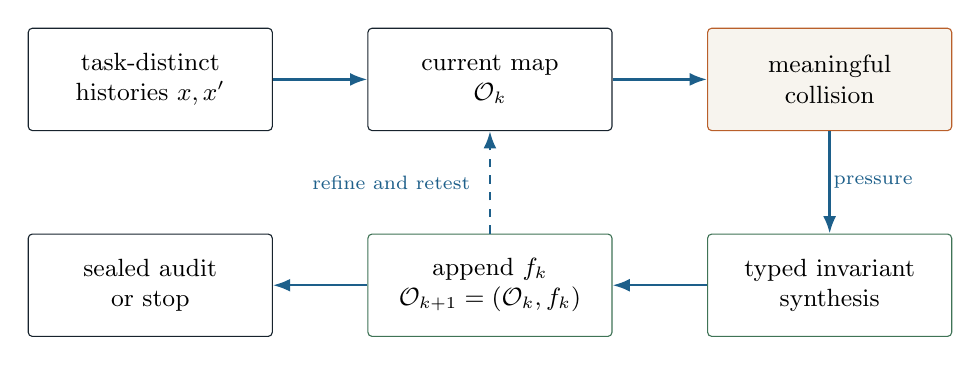
\begin{tikzpicture}[
  node distance=10mm and 12mm,
  every node/.style={font=\small,align=center},
  box/.style={draw=vdink,rounded corners=1.5pt,minimum height=13mm,minimum width=31mm,fill=white},
  pressure/.style={box,draw=vdorange,fill=vdcream},
  repair/.style={box,draw=vdgreen,fill=white},
  arrow/.style={-{Latex[length=2.2mm]},line width=0.9pt,color=vdblue}
]
\node[box] (history) {task-distinct\\histories $x,x'$};
\node[box,right=of history] (obs) {current map\\$\Obs_k$};
\node[pressure,right=of obs] (collision) {meaningful\\collision};
\node[repair,below=13mm of collision] (synth) {typed invariant\\synthesis};
\node[repair,left=of synth] (append) {append $f_k$\\$\Obs_{k+1}=(\Obs_k,f_k)$};
\node[box,left=of append] (audit) {sealed audit\\or stop};
\draw[arrow] (history) -- (obs);
\draw[arrow] (obs) -- (collision);
\draw[arrow] (collision) -- node[right,font=\scriptsize,fill=white,inner sep=1pt]{pressure} (synth);
\draw[arrow] (synth) -- (append);
\draw[arrow] (append) -- (audit);
\draw[arrow,dashed] (append.north) --
  node[midway,left=2mm,font=\scriptsize,fill=white,inner sep=1pt]{refine and retest}
  (obs.south);
\end{tikzpicture}
\end{center}
\vfill

\fcolorbox{vdink}{vdpale}{%
\begin{minipage}{0.94\linewidth}
\textbf{Evidence statement.}
The partition-refinement, finite-sample completion, threshold-nesting, and similarity-invariance results are proved under explicit assumptions. The reported numerical values are deterministic computations or internally frozen holdout audits. Three independently seeded synthetic domains show collision-risk reductions; two real UCR test sets do not establish significant transfer. The study is not externally preregistered, does not prove population injectivity, and does not claim discovery of a physical conservation law.
\end{minipage}}

\vspace{0.30in}
\noindent{\color{vdblue}\rule{\linewidth}{0.8pt}}
\end{titlepage}
\hypersetup{pageanchor=true}

\begin{abstract}
Papers I and II hold the representation fixed: the first asks when dynamics and observation preserve distinctions, and the second asks whether a distinction hidden inside one representation fibre can matter for a future prediction. This paper makes the representation itself dynamic. A \emph{meaningful collision} occurs when two task-distinct trajectories remain close under the current observation map. Such collisions become counterexamples that pressure a constrained search to synthesize a unary observable and append it to the map.

The mathematical core is simple but consequential. Exact append-only augmentation refines observation fibres; on a finite sample, a separator-complete search reaches injectivity in at most the number of unresolved class splits; and a fixed max-product metric makes threshold-collision sets nested. For trajectories transformed by translation, positive global scale, and orthogonal channel action, global RMS canonicalization and quantile recurrence preserve adjacency exactly outside deterministic tie pathologies. The resulting primitive library combines temporal, covariance, recurrence-network, and persistent-homology summaries. A depth-two typed grammar produces 271 auditable scalar programs.

The executable audit uses logistic, Lorenz, and Kuramoto systems. Programs are selected on two source domains, frozen before independent audit trajectories are materialized, and evaluated on 120 disjoint cross-label pairs from the held-out system. Collision risk falls from $0.992$ to $0$ for logistic, $0.917$ to $0.467$ for Lorenz, and $1$ to $0.083$ for Kuramoto; the macro absolute reduction is $0.786$. A full-pipeline 99-permutation source-label null selects no program in every fold. An explicitly post-hoc phase audit links the $N=5$ Kuramoto winner to latent second-harmonic coherence ($\rho_S=0.907$; $0.944$ within weak coupling) without upgrading the held-out claim. Yet an admissible random-program comparator is beaten significantly only for Kuramoto, and the all-source expression fails to transfer significantly to ECGFiveDays or Earthquakes. The result is therefore a verified mechanism for constrained representation repair in controlled domains, not a universal invariant-discovery claim.
\end{abstract}

\claimbox{Primary result}{Meaningful representation collisions can be converted into counterexamples for a typed, nuisance-invariant synthesis loop. In the released implementation, one scalar program is actually reinserted into the observation map and substantially reduces collision risk across three independent synthetic audits. The exact refinement guarantees are structural; empirical transfer beyond those controlled systems remains open.}

\setcounter{tocdepth}{1}
{\small\tableofcontents}
\clearpage

\section{The third move: make representation dynamic}

\subsection{One problem, three directions}

Voss Dynamics studies what happens to information-bearing distinctions under physical evolution and representation. Paper I asks whether a distinction between possible states or histories survives a dynamical map and a fixed observation map. Paper II asks whether two histories merged by that map can still imply different future observations. This paper begins after a predictive witness has made that failure operational: if the current map is insufficient, how should it change?

The proposed answer is not to increase dimension blindly. It is to use the failed fibre as a counterexample, search a predeclared library for a compact coordinate that separates it, reject coordinates that respond to declared nuisance transformations, append the winner, and retest. ``Pressure'' names this counterexample signal. It is not thermodynamic pressure. ``Invariant'' means invariance to a declared nuisance group. It does not mean that the synthesized observable is conserved along the physical flow.

The relation to observability is direct. Classical nonlinear observability asks whether a state can be reconstructed from an output history \citep{HermannKrener1977}; delay embedding supplies generic reconstruction results under smooth noiseless hypotheses \citep{Takens1981,Sauer1991}. Here the object is narrower and more operational: a finite, task-indexed representation is repaired when it merges distinctions that a declared witness says matter.

\subsection{Claim discipline}

Four statuses are used throughout:
\begin{description}[
  style=multiline,
  leftmargin=7.25em,
  labelwidth=6.4em,
  labelsep=0.55em
]
\item[\status{PROVED}:] A mathematical consequence of explicitly stated assumptions.
\item[\status{COMPUTED}:] A deterministic symbolic or numerical check reproduced by the evidence package.
\item[\status{HELD-OUT}:] A result on data not used by the final in-run selection step. This is internal freezing, not external preregistration or independent replication.
\item[\status{OPEN}:] A claim requiring new domains, prospective commitment, physical data, or stronger theory.
\end{description}
The complete claim ledger is supplied beside the manuscript. The release also records an earlier development failure: a first version admitted programs under permuted source labels. Gates were then strengthened, final audit seeds were changed, and the final run was executed. That history makes the final audit useful but not prospective confirmation.

\subsection{The six gates}

\begin{table}[H]
\centering
\caption{The six gates of Paper III. Passing an earlier gate does not imply passage of a later one.}
\label{tab:gates}
\small
\begin{tabularx}{\linewidth}{@{}p{0.07\linewidth}X p{0.28\linewidth}@{}}
\toprule
Gate & Requirement & Present result\\
\midrule
1 & Define task distinction, collision geometry, nuisance group, and claim scope. & \status{PROVED/DECLARED}: formal objects fixed in \cref{sec:formal}.\\
2 & Show that augmentation truly refines the representation. & \status{PROVED}: exact refinement, finite completion, and threshold nesting.\\
3 & Construct interpretable unary coordinates with auditable invariance. & \status{PROVED/COMPUTED}: similarity group, recurrence theorem, 24/24 adjacency checks.\\
4 & Search, select, and actually reinsert a coordinate under fixed gates. & \status{COMPUTED}: 271-program grammar; explicit append-only implementation.\\
5 & Survive independent controlled audits and complete-pipeline nulls. & \status{HELD-OUT}: three synthetic domains; no selection in $0/99$ source-label permutations per fold.\\
6 & Transfer without adaptation to real data. & \status{OPEN}: neither real UCR stress test is significant.\\
\bottomrule
\end{tabularx}
\end{table}

\section{Meaningful collisions and representation pressure}
\label{sec:formal}

\subsection{Domains, distinctions, and fibres}

Let $d\in\cD$ index a domain, $x\in\cX_d$ a finite trajectory, and
\begin{equation}
  \Obs_k:\cX_d\longrightarrow\R^{m_k}
  \label{eq:observation-map}
\end{equation}
the representation after $k$ successful additions. Exact equality under $\Obs_k$ induces the fibre relation
\begin{equation}
  x\sim_k x' \quad\Longleftrightarrow\quad \Obs_k(x)=\Obs_k(x').
\end{equation}
A task witness declares whether their difference matters:
\begin{equation}
  D_d(x,x')
  =\ind\{\ell_d(x,x')>\delta_d\}.
  \label{eq:distinction}
\end{equation}
The witness may encode a latent regime, a known parameter interval, a future-outcome difference, or a label mismatch. Without such a witness, every discrepancy due to measurement noise would count as a distinction, and ``collision'' would be scientifically underdetermined.

For the executable binary benchmarks, $D_d(x,x')=1$ exactly when labels differ. Each coordinate is passed through the fixed source-independent squash
\begin{equation}
  h(z)=\frac{2}{\pi}\arctan z,
\end{equation}
and the representation distance is
\begin{equation}
  d_k(x,x')
  =\max_{1\le j\le m_k}
  \left|h(\Obs_{k,j}(x))-h(\Obs_{k,j}(x'))\right|.
  \label{eq:max-metric}
\end{equation}
At a fixed threshold $\tau$, define the meaningful-collision indicator and its conditional risk:
\begin{align}
  C_{k,\tau}(x,x')
  &=\ind\{D_d(x,x')=1,\ d_k(x,x')\le\tau\},
  \label{eq:collision}\\
  R_{d,k}(\tau)
  &=\Prob_d\!\left(d_k(X,X')\le\tau\given D_d(X,X')=1\right).
  \label{eq:risk}
\end{align}
The benchmark fixes $\tau=0.22$. Absolute reduction,
\begin{equation}
  \Delta R_d(f)=R_{d,k}(\tau)-R_{d,k+1}(\tau),
  \label{eq:absolute-reduction}
\end{equation}
is primary. Relative reduction is unstable when the baseline risk is small.

\subsection{Pressure is a counterexample, not a metaphorical score}

A sampled pair with $C_{k,\tau}=1$ is a concrete counterexample to sufficiency at resolution $\tau$. It says that the current coordinates cannot separate this task-distinct pair. A candidate must be a \emph{unary} map $f:\cX_d\to\R$: pairwise diagnostics such as $g(x-x')$ cannot literally be appended to a per-trajectory representation unless converted through fixed landmarks or a declared kernel construction.

The update is
\begin{equation}
  \Obs_{k+1}(x)=\bigl(\Obs_k(x),f_k(x)\bigr).
  \label{eq:append}
\end{equation}
That one line is the architectural hinge. A legacy prototype placed synthesized pairwise functions in a registry but never appended their values to $\Obs_k$. The released engine tests the resulting matrix dimension and the appended column directly.

\subsection{Declared nuisance group}

For a $T\times p$ trajectory matrix $X$, the implemented nuisance group is
\begin{equation}
  g\cdot X=aXQ+\bm1 b^\mathsf T,
  \qquad a>0,\quad Q\in O(p),\quad b\in\R^p.
  \label{eq:nuisance-group}
\end{equation}
Translation, positive global scale, and orthogonal channel mixing model changes of offset, units, and sensor basis that should not change the chosen observable. Anisotropic scaling, nonlinear sensor response, time warping, resampling, and missingness are not in this group. Their treatment is empirical robustness, not exact invariance.

\section{What augmentation guarantees}
\label{sec:theorems}

\begin{theorem}[Exact fibre refinement]
\label{thm:refinement}
Let $\Obs_{k+1}=(\Obs_k,f)$. Then every $\Obs_{k+1}$-fibre is contained in an $\Obs_k$-fibre. The refinement is strict if and only if $f$ is nonconstant on at least one $\Obs_k$-fibre.
\end{theorem}

\begin{proof}
If $\Obs_{k+1}(x)=\Obs_{k+1}(x')$, equality of the first block gives $\Obs_k(x)=\Obs_k(x')$. Thus $\sim_{k+1}$ implies $\sim_k$. Strictness occurs exactly when some pair with $x\sim_k x'$ has $f(x)\ne f(x')$.
\end{proof}

\begin{theorem}[Conditional finite-sample completion]
\label{thm:completion}
Let a finite sample $S$ contain $n$ distinct trajectories, and suppose $\Obs_0$ induces $c_0$ nonempty equivalence classes on $S$. If, whenever the current partition is not discrete, the hypothesis class contains a unary candidate that splits at least one nonsingleton fibre and the search returns such a candidate, then append-only synthesis makes $\Obs_k$ injective on $S$ after at most $n-c_0$ successful additions.
\end{theorem}

\begin{proof}
By \cref{thm:refinement}, no current class can merge with another. Every successful candidate splits at least one class and therefore increases the number of nonempty classes by at least one. A partition of $n$ objects has at most $n$ classes. Hence at most $n-c_0$ increases are required.
\end{proof}

\begin{remark}
The theorem is conditional and finite-sample. It does not prove population injectivity, global nonlinear observability, separator completeness of a practical grammar, or successful search under noise. A zero collision count on a finite audit is not an injectivity theorem.
\end{remark}

\begin{theorem}[Nested threshold collisions]
\label{thm:nesting}
Fix $\tau$ and the coordinate transform $h$. If $d_k$ is the max metric in \cref{eq:max-metric} and $\Obs_{k+1}=(\Obs_k,f)$, then
\begin{equation}
  \{(x,x'):C_{k+1,\tau}(x,x')=1\}
  \subseteq
  \{(x,x'):C_{k,\tau}(x,x')=1\}.
  \label{eq:nesting}
\end{equation}
Consequently empirical collision risk on any fixed set of distinct pairs cannot increase after an append-only update.
\end{theorem}

\begin{proof}
The new distance is
\[
d_{k+1}(x,x')=\max\{d_k(x,x'),|h(f(x))-h(f(x'))|\}\ge d_k(x,x').
\]
Therefore $d_{k+1}\le\tau$ implies $d_k\le\tau$. The task witness $D_d$ is unchanged.
\end{proof}

Re-estimating a rank transform on held-out data, rescaling old coordinates after every round, changing $\tau$, or replacing the max metric can invalidate \cref{thm:nesting}. The implementation uses one fixed analytic squash precisely to avoid those loopholes.

\subsection{Risk statements require independent units}

All $\binom n2$ pairs from $n$ trajectories are dependent. Treating them as independent Bernoulli trials would manufacture confidence. The outer audit therefore shuffles each binary class once and makes disjoint cross-class matches, so each trajectory contributes to at most one trial.

\begin{proposition}[Exact upper bound after zero collisions]
\label{prop:zero-bound}
For $K$ independent Bernoulli collision trials and zero observed collisions, the exact one-sided $(1-\alpha)$ Clopper--Pearson upper bound is
\begin{equation}
  p_U=1-\alpha^{1/K}.
  \label{eq:cp}
\end{equation}
\end{proposition}

At 95\% confidence, $K=120$ zero-collision trials yield $p_U=0.0247$; approximately 299, 2,995, and 29,956 independent pairs are required to bound risk below $10^{-2}$, $10^{-3}$, and $10^{-4}$, respectively \citep{ClopperPearson1934}. Pairwise source selection may use the full cross-label array as a dependent U-statistic, but outer uncertainty must respect its dependence structure \citep{Hoeffding1948}.

\begin{proposition}[Finite-grammar audit bound]
\label{prop:grammar-bound}
For a fixed finite grammar $\cH$ with $|\cH|=M$ and $K$ independent audit pairs, Hoeffding's inequality and a union bound give, with probability at least $1-\alpha$,
\begin{equation}
  \sup_{f\in\cH}|\widehat R(f)-R(f)|
  \le
  \sqrt{\frac{\log(2M/\alpha)}{2K}}.
  \label{eq:finite-bound}
\end{equation}
\end{proposition}

This bound is intentionally conservative and applies only if the grammar and audit are genuinely fixed. It is not used to relabel the internally frozen experiment as prospective evidence.

\section{Canonical structure without false completeness}
\label{sec:canonical}

\subsection{Global canonicalization}

For a trajectory $X\in\R^{T\times p}$ define
\begin{equation}
  \widetilde X
  =\frac{X-\bm1\bar x^\mathsf T}
  {\sqrt{T^{-1}\|X-\bm1\bar x^\mathsf T\|_F^2}},
  \label{eq:normalize}
\end{equation}
with the zero trajectory returned when the denominator is numerically zero. A delay cloud concatenates three copies at lags $0,2,4$ and deterministically subsamples at most 72 points. All distance geometry is computed from this cloud.

\begin{theorem}[Similarity equivariance of the normalized cloud]
\label{thm:similarity}
For $g$ in \cref{eq:nuisance-group}, nonconstant $X$ obeys
\begin{equation}
  \widetilde{(g\cdot X)}=\widetilde XQ.
\end{equation}
Consequently all Euclidean pairwise distances in the corresponding delay cloud are unchanged.
\end{theorem}

\begin{proof}
Centering removes $b$. Orthogonality preserves the Frobenius norm, and $a>0$ cancels between numerator and denominator. Delay concatenation applies the block-orthogonal action $\operatorname{diag}(Q,Q,Q)$, which preserves pairwise Euclidean distances.
\end{proof}

\subsection{Quantile recurrence}

Let $d_{ij}$ be delay-cloud distances and let $\epsilon_q$ be their empirical $q$-quantile for $i<j$. With $q=0.12$, define
\begin{equation}
  A_{ij}=\ind\{i\ne j,\ d_{ij}\le\epsilon_q\}.
  \label{eq:recurrence}
\end{equation}

\begin{corollary}[Quantile-recurrence invariance]
\label{cor:recurrence}
Under the nuisance group in \cref{eq:nuisance-group}, $A$ is unchanged under a fixed deterministic quantile and tie rule. Degree summaries, transitivity, and normalized-Laplacian spectra therefore inherit the same invariance.
\end{corollary}

The implementation checks 24 transformed trajectories and obtains identical adjacency matrices in all 24 cases. It also tests normalized-Laplacian indexing on two known graphs: $\lambda_2(P_4)=0.5$, while disconnected $2P_2$ has $\lambda_2=0$. This matters because selecting the second \emph{positive} eigenvalue silently returns $\lambda_3$ and can report nonzero ``connectivity'' for a disconnected graph.

\subsection{Recurrence is discontinuous at the threshold}

Exact invariance to the declared group is not general perturbation stability. If a perturbation changes each distance by at most $\eta_d$ and moves the empirical threshold by at most $\eta_q$, only pairs satisfying
\begin{equation}
  |d_{ij}-\epsilon_q|>\eta_d+\eta_q
  \label{eq:margin}
\end{equation}
are guaranteed to preserve edge status. Near-threshold edges may flip. A quantile construction also makes edge density nearly fixed, so raw density and mean degree are omitted as informative candidates; degree variation and higher-order structure remain.

\subsection{Topology and temporal coordinates}

Finite $H_0$ lifetimes are minimum-spanning-tree edge lengths, normalized by median pairwise distance. $H_1$ lifetimes are computed by Vietoris--Rips persistence and normalized by the same source-independent geometric scale. Persistence diagrams are stable under metric perturbation \citep{CohenSteiner2007,Chazal2014}; stable vector summaries such as landscapes and images are established alternatives \citep{Bubenik2015,Adams2017}. Stability does not imply discriminative completeness.

The primitive library contains 18 total coordinates, of which two form the initial representation and 16 enter the grammar:
\begin{itemize}
\item recurrence $\lambda_2$, $\lambda_3$, spectral entropy, degree coefficient of variation, and transitivity;
\item normalized $H_0$ total, maximum, and entropy, plus $H_1$ count, maximum, and total persistence;
\item radial spectral entropy, radial permutation entropy, radial turning rate, increment coefficient of variation, and covariance-spectrum entropy.
\end{itemize}
The baseline coordinates are radial lag-one correlation and path tortuosity.

\warningbox{Noncompleteness is explicit}{A logistic trajectory and its time reversal are different oriented histories, yet their recurrence normalized-Laplacian spectra agree to $3.83\times10^{-15}$. Graph spectra can be cospectral, persistence summaries can collide, and nuisance invariance necessarily discards information. The canonical field is a constrained representation, not a complete coordinate system.}

\section{The synthesis engine}
\label{sec:engine}

\subsection{A finite typed grammar}

Every candidate maps one trajectory to one scalar. The depth-two grammar contains:
\begin{align}
  f(x)&=u_i(x),\\
  f(x)&=\frac{u_i(x)-u_j(x)}{|u_i(x)|+|u_j(x)|+10^{-9}},\\
  f(x)&=\log\frac{|u_i(x)|+10^{-9}}{|u_j(x)|+10^{-9}},\\
  f(x)&=\operatorname{sgn}(u_i u_j)\sqrt{|u_i u_j|}.
\end{align}
Primitive complexity is one; a binary expression has complexity three. Geometric means are restricted to adjacent primitives in deterministic sorted order. The resulting manifest contains 271 programs. Protected operations return finite values and clip only beyond magnitude $10^6$.

This is symbolic feature construction, but its objective differs from ordinary equation fitting. Symbolic regression searches for compact relations in data \citep{SchmidtLipson2009,Udrescu2020}; SINDy searches sparse governing equations \citep{Brunton2016}. Here the output is an observation coordinate chosen to split counterexample fibres while surviving a nuisance gate.

\subsection{Selection rule}

Within each source domain, records are stratified into 60\% selection and 40\% audit subsets. A candidate must satisfy, across every source domain:
\begin{align}
  e_{\rm inv}(f)&\le5\times10^{-6},\\
  Q_{0.95}\bigl[e_{\rm noise}(f)\bigr]&\le0.20,\\
  \min_d\Delta R_d^{\rm audit}(f)&\ge0.15,\\
  \min_d\operatorname{AUC}^{\rm audit}_{\pm}(f)&\ge0.75,\\
  \min_d\operatorname{AUC}^{\rm select}_{\pm}(f)&\ge0.70,
  \label{eq:gates}
\end{align}
where orientation-free AUC is $\max(\operatorname{AUC},1-\operatorname{AUC})$. Surviving candidates are ordered deterministically by
\begin{align}
  U(f)=&\ \min_d\Delta R_d^{\rm audit}
  +0.50\,\operatorname{mean}_d\Delta R_d^{\rm audit}
  +0.15\min_d\Delta R_d^{\rm select}\nonumber\\
  &+0.05\bigl(\operatorname{mean}_d\operatorname{AUC}^{\rm audit}_{\pm}-0.5\bigr)
  -0.003\,\operatorname{complexity}(f)
  -0.10\,Q_{0.95}[e_{\rm noise}(f)].
  \label{eq:utility}
\end{align}
The winner is appended, never substituted for an old coordinate. Search stops when no candidate passes or after three additions. In the released runs it stops after one.

\subsection{Executable loop}

\begin{figure}[H]
\centering
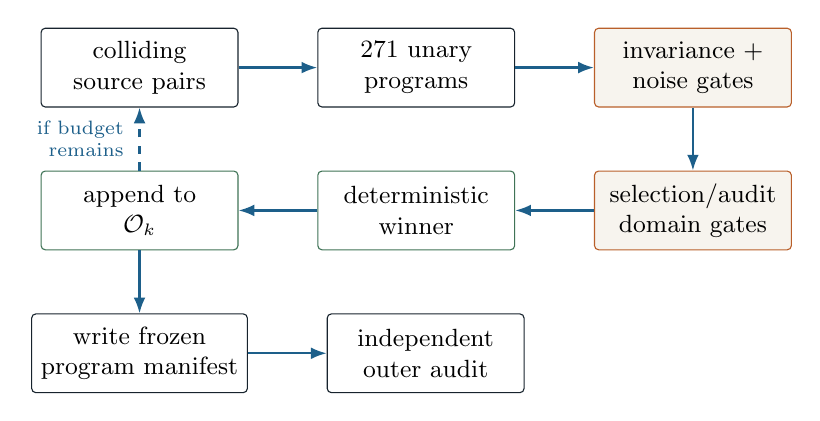
\begin{tikzpicture}[
  node distance=8mm and 10mm,
  every node/.style={font=\small,align=center},
  stage/.style={draw=vdink,rounded corners=1.5pt,minimum height=10mm,minimum width=25mm,fill=white},
  gate/.style={stage,draw=vdorange,fill=vdcream},
  pass/.style={stage,draw=vdgreen},
  arrow/.style={-{Latex[length=2mm]},line width=0.8pt,color=vdblue}
]
\node[stage] (pairs) {colliding\\source pairs};
\node[stage,right=of pairs] (grammar) {271 unary\\programs};
\node[gate,right=of grammar] (invariance) {invariance +\\noise gates};
\node[gate,below=of invariance] (inner) {selection/audit\\domain gates};
\node[pass,left=of inner] (winner) {deterministic\\winner};
\node[pass,left=of winner] (reinsert) {append to\\$\Obs_k$};
\node[stage,below=of reinsert] (freeze) {write frozen\\program manifest};
\node[stage,right=of freeze] (outer) {independent\\outer audit};
\draw[arrow] (pairs) -- (grammar);
\draw[arrow] (grammar) -- (invariance);
\draw[arrow] (invariance) -- (inner);
\draw[arrow] (inner) -- (winner);
\draw[arrow] (winner) -- (reinsert);
\draw[arrow,dashed] (reinsert.north) -- node[midway,left=2pt,font=\scriptsize,align=right]{if budget\\remains} (pairs.south);
\draw[arrow] (reinsert) -- (freeze);
\draw[arrow] (freeze) -- (outer);
\end{tikzpicture}
\caption{The pressure loop. Source pairs drive candidate choice; the program, preprocessing, threshold, and split declaration are serialized before independent synthetic audit and real-test loading within the final run. The freeze has no external timestamp.}
\label{fig:loop}
\end{figure}

The selected all-source program is
\begin{equation}
  \program(X)=
  \log\frac{\operatorname{CV}(\|\Delta\widetilde X_t\|)+10^{-9}}
  {H_{\rm perm}(\|\widetilde X_t\|)+10^{-9}},
  \label{eq:selected}
\end{equation}
the log ratio of increment coefficient of variation to radial permutation entropy. Its maximum relative discrepancy under the declared similarity transform is $2.58\times10^{-14}$ over every trajectory in the final suite.

\subsection{Why the replacement engine was necessary}

The historical prototype contributed the conceptual loop but not valid evidence. Forensic recovery showed that its synthesized feature was not reinserted; it mixed unary and pairwise programs; indexed recurrence connectivity incorrectly; used one perturbation so a variance-based stability score was identically one; and allowed nominal transfer domains into optimization. Its retained seismic pilot additionally lacks raw data and contains target-selection and normalization leakage. All legacy quantitative claims are excluded. The release preserves the exact commit and defects in a dedicated audit so that the development path is inspectable rather than erased.

\section{Evidence contract}
\label{sec:protocol}

\subsection{Controlled discovery and independent audit}

The discovery suite has three qualitatively different generators, using canonical logistic, Lorenz, and coupled-oscillator models as controlled test beds \citep{May1976,Lorenz1963,Kuramoto1975}:
\begin{itemize}
\item \textbf{Logistic:} $r\in[3.20,3.42]$ versus $r\in[3.90,3.99]$, 256 retained scalar samples after burn-in, Gaussian noise $\sigma=0.003$.
\item \textbf{Lorenz:} $\rho\in[17,21]$ versus $\rho\in[27,31]$, RK4 at $\Delta t=0.008$, 256 retained three-channel samples, Gaussian noise $\sigma=0.01$.
\item \textbf{Kuramoto:} five oscillators with coupling $K\in[2.8,4.0]$ versus $K\in[0.05,0.45]$, 256 retained sine-channel samples, Gaussian noise $\sigma=0.015$.
\end{itemize}
Discovery uses 28 trajectories per class per system. For each outer fold, two systems are sources. The held-out system is regenerated after program freeze with a separate final seed and 120 trajectories per class. One random matching creates 120 disjoint cross-label pairs. No audit trajectory participates in source feature scaling, grammar construction, candidate gates, or stopping.

The two baseline features, fixed squash, $\tau=0.22$, group action, 271-program grammar, three-round budget, and gate constants are machine-readable. Source selection uses all cross-label pairs only inside source data. The outer statistic uses independent matched pairs and a paired 4,000-repetition bootstrap on before/after indicators.

\subsection{Nulls and ablations}

Three different controls answer different questions:
\begin{enumerate}
\item \textbf{Fixed-program label permutation:} permute audit labels 999 times while holding the chosen program fixed.
\item \textbf{Full-pipeline source-label null:} permute source labels, rerun all synthesis gates, then apply any selected program to the untouched independent audit. Ninety-nine repetitions set a minimum attainable $p$-value of $0.01$ using the plus-one rule \citep{PhipsonSmyth2010}.
\item \textbf{Admissible random-program comparator:} draw one program that passes source invariance and noise gates, apply it directly to the outer audit, and repeat 999 times. This is not a rerun of source-domain selection and is not described as equal-compute.
\end{enumerate}
Primitive-only, recurrence-only, and topology-only grammars are rerun through the same one-round source selection. Phase-randomized and IAAFT surrogates \citep{Theiler1992,SchreiberSchmitz1996}, time warps, irregular sampling, and full learned-representation baselines remain specified extensions rather than completed evidence.

\subsection{Real-data stress, sealed only within the run}

After the all-source program is serialized, the runner reads only the official UCR archive \texttt{TEST} members for ECGFiveDays and Earthquakes \citep{Dau2019}. It deterministically samples up to 32 cases per class, producing 64 trajectories and 32 disjoint cross-label pairs per dataset. Archive SHA-256 digests, exact selected identifiers, and acquisition URLs are shipped. No real record changes the expression, constants, threshold, or preprocessing.

This is a stringent zero-adaptation stress test but not a prospective registered study. The task meanings also differ: ECG morphology and a constructed earthquake-event classification problem are not draws from a well-defined population of ``all dynamical systems.'' Results are therefore reported by name, not generalized to an imaginary superpopulation.

\section{Results}
\label{sec:results}

\subsection{Independent synthetic audits}

\begin{table}[H]
\centering
\caption{Independent synthetic audit. Each row uses 120 disjoint cross-label pairs generated with a seed not used in discovery. Intervals are paired bootstrap 95\% intervals for absolute reduction.}
\label{tab:synthetic}
\small
\begin{tabularx}{\linewidth}{@{}lrrrrrX@{}}
\toprule
Held out & Before & After & $\Delta R$ & 95\% interval & AUC & Selected program\\
\midrule
Logistic & 0.992 & 0.000 & 0.992 & [0.975, 1.000] & 1.000 & $\log(\mathrm{increment\ CV}/\mathrm{radial\ PE})$\\
Lorenz & 0.917 & 0.467 & 0.450 & [0.358, 0.533] & 0.828 & $\log(\mathrm{covariance\ entropy}/H_1\mathrm{\ max})$\\
Kuramoto & 1.000 & 0.083 & 0.917 & [0.867, 0.967] & 0.998 & $\log(\mathrm{increment\ CV}/\mathrm{radial\ PE})$\\
\midrule
Macro mean & 0.969 & 0.183 & 0.786 & --- & 0.942 & fold-specific frozen programs\\
\bottomrule
\end{tabularx}
\end{table}

The logistic fold has zero post-repair collisions, giving a one-sided exact 95\% upper risk bound of $0.0247$, not zero population risk. Lorenz retains 56/120 collisions and is the clearest controlled failure mode. Kuramoto retains 10/120. All three fixed-program permutation values are below $0.05$ ($0.001$, $0.027$, and $0.001$ for logistic, Lorenz, and Kuramoto). More importantly, the full source-label pipeline selects no program in $0/99$ permutations for each fold; the plus-one $p$-value is $0.01$.

\begin{figure}[H]
\centering
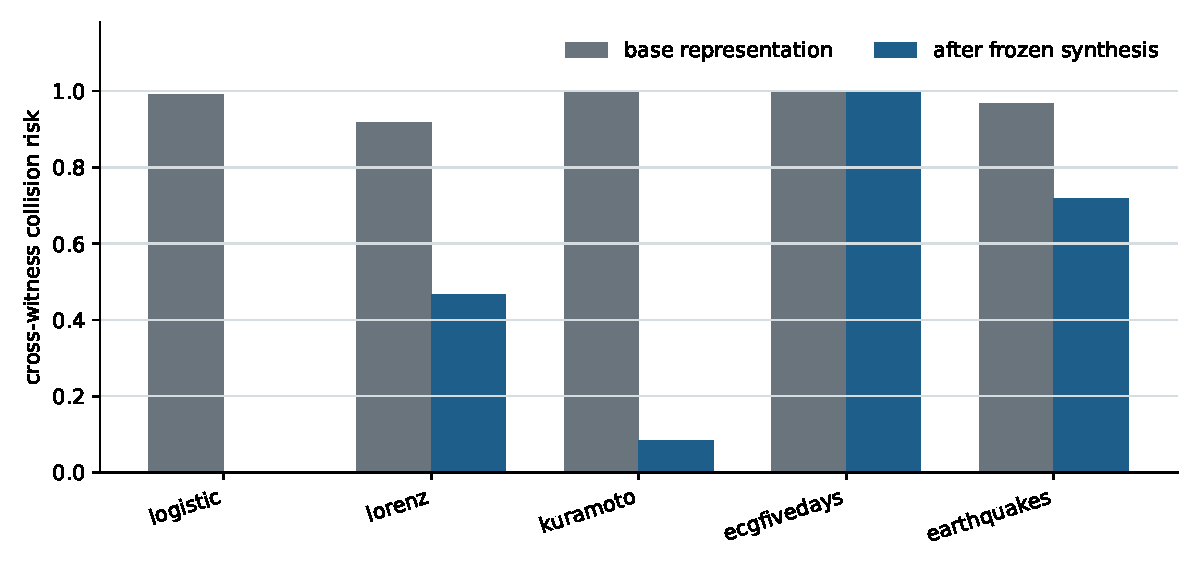
\includegraphics[width=0.93\linewidth]{frozen_transfer.pdf}
\caption{Cross-witness collision risk before and after the frozen fold-specific program for controlled synthetic audits (first three groups), followed by the all-source program on two real UCR stress tests. The visual discontinuity is substantive: strong controlled-domain repair does not imply real-domain transfer.}
\label{fig:transfer}
\end{figure}

\subsection{The random-program comparator and ablations}

The selected program exceeds the admissible random-program distribution significantly only for Kuramoto: comparator $p$-values are $0.119$ for logistic, $0.166$ for Lorenz, and $0.034$ for Kuramoto. Therefore the data support successful gated synthesis, but not systematic superiority over a randomly drawn admissible grammar member across all three domains.

\begin{table}[H]
\centering
\caption{Absolute collision-risk reduction under one-round grammar ablations on the independent synthetic audits. A zero may mean no program passed the source gates.}
\label{tab:ablations}
\small
\begin{tabular}{@{}lrrrr@{}}
\toprule
Held out & Full grammar & Primitive only & Recurrence only & Topology only\\
\midrule
Logistic & 0.992 & 0.000 & 0.133 & 0.000\\
Lorenz & 0.450 & 0.133 & 0.000 & 0.383\\
Kuramoto & 0.917 & 0.000 & 0.000 & 0.292\\
\bottomrule
\end{tabular}
\end{table}

No single family dominates every system. Under these source-selection gates, the symbolic composition is essential to transfer into logistic and Kuramoto, while a topology-only expression approaches the full Lorenz reduction. This supports a heterogeneous primitive library; it does not establish that these are optimal primitives or that the selected composition is the only target-domain separator.

\subsection{A post hoc mechanistic read of the Kuramoto fold}
\label{sec:kuramoto-posthoc}

\status{COMPUTED; POST HOC}. Kuramoto is the only fold in which the source-selected expression significantly exceeds the admissible random-program comparator. The winner was chosen from logistic and Lorenz records and frozen before any Kuramoto audit trajectory was generated. After that result was known, the exact 240-record audit was regenerated bit-for-bit---the maximum observed-channel discrepancy is zero---while retaining latent phases that were never exposed to synthesis.

For the conventional generalized order parameters and their time averages, define \citep{Daido1992}
\begin{equation}
  Z_m(t)=\frac{1}{N}\sum_{j=1}^{N}e^{im\theta_j(t)},
  \qquad
  \overline R_m=\frac{1}{T}\sum_t |Z_m(t)|.
  \label{eq:kuramoto-order}
\end{equation}
The noiseless sine sensor vector $s_j(t)=\sin\theta_j(t)$ obeys the exact identity
\begin{equation}
  \|s(t)\|_2^2=\frac{N}{2}\bigl[1-\Re Z_2(t)\bigr].
  \label{eq:sine-order}
\end{equation}
The released observed array adds Gaussian measurement noise after this sine transform, so \cref{eq:sine-order} is not an exact identity for the array supplied to synthesis. Even without that noise, channel centering adds the explicit correction $-2\sum_j\bar s_j\sin\theta_j(t)+\sum_j\bar s_j^2$, after which the declared global RMS normalization is applied. The identity therefore supplies a mechanistic route by which radial permutation entropy can remain sensitive to generalized phase-order structure, while increment CV summarizes temporal heterogeneity of the multichannel motion. It does not identify the computed feature with $Z_1$ or $Z_2$.

On the exact audit, the frozen scalar has orientation-free label AUC $0.9976$; latent $\overline R_1$ and $\overline R_2$ each have AUC $0.9989$. The scalar's pooled Spearman correlation is $0.861$ with $\overline R_1$ (stratified record-bootstrap 95\% interval $[0.833,0.885]$) and $0.907$ with $\overline R_2$ (interval $[0.885,0.927]$). The second-harmonic association sharpens within the weak-coupling class: $\rho_S=0.944$ (record-bootstrap interval $[0.908,0.963]$), versus $0.888$ for increment CV and $-0.864$ for radial permutation entropy. In a paired record bootstrap, the composite-minus-increment correlation difference is $0.056$ ($[0.029,0.095]$), and the composite-minus-oriented-entropy difference is $0.080$ ($[0.043,0.128]$). These intervals were designed after inspection and are descriptive, not confirmatory.

This is a narrow within-regime gain, not evidence that symbolic composition is required for the coarse target contrast. Across the two widely separated coupling classes, increment CV alone has AUC $0.9992$, slightly above the composite. Its primitive-only ablation failed the \emph{source} gates; it was not intrinsically uninformative on Kuramoto. The multichannel relation is nevertheless essential to the released scalar: after recomputing canonicalization and both primitives for every one of the $\binom{5}{m}$ channel subsets, mean label AUC rises from $0.522$ for one channel to $0.950$, $0.992$, $0.998$, and $0.998$ for two through five channels.

\begin{figure}[H]
\centering
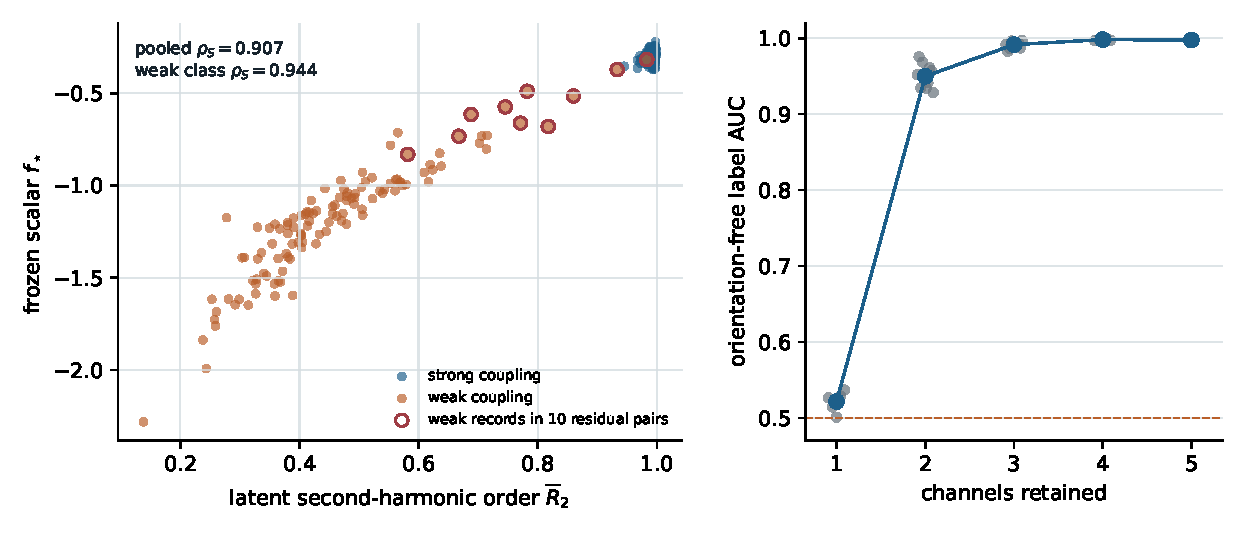
\includegraphics[width=0.94\linewidth]{kuramoto_posthoc.pdf}
\caption{Post-hoc interpretation of the frozen Kuramoto winner. Left: the source-selected scalar tracks latent second-harmonic coherence $\overline R_2$; rings mark the weak-coupling records in the ten residual released-match collisions. Right: every point is one of the $\binom{5}{m}$ channel subsets, with canonicalization and both primitives recomputed for that subset; blue points are subset-count means. These are descriptive diagnostics on a result already seen, not a new held-out test.}
\label{fig:kuramoto-posthoc}
\end{figure}

The ten weak-coupling records in the residual released matching are unusually ordered within their declared class: mean $\overline R_1$ is $0.874$, versus $0.570$ for the other weak-coupling records, while mean $K$ is $0.346$ versus $0.237$. The conclusion is not an accident of one matching: all $14{,}400$ cross-label pairs have post-repair risk $0.091$, and 20,000 random perfect matchings give a descriptive 95\% risk range $[0.075,0.108]$; the released $10/120=0.083$ lies inside it.

The bounded interpretation is therefore that a scalar selected without Kuramoto access transferred as an order-sensitive, sensor-basis-invariant surrogate inside this finite controlled generator. Its strongest post-hoc association is with generalized second-harmonic coherence, and the ratio combines complementary temporal signals for within-weak-class ranking. The analysis is post hoc, $N=5$, the coupling intervals are widely separated, the expression's orientation reverses across other systems, and a simpler target-domain primitive separates the coarse classes at least as well. It is not a conserved invariant, a critical-coupling estimate, a universal order coordinate, or evidence of information beyond conventional order summaries.

\subsection{Invariance and robustness audits}

The all-source expression in \cref{eq:selected} passes its source selection noise gate with 95th-percentile relative error $0.110<0.20$. Across synthetic audits and both real sets, however, the same statistic has median error $0.034$, 95th percentile $0.265$, and maximum $0.415$ under 2\% relative Gaussian perturbations. The source gate therefore does not guarantee unseen-domain robustness. Exact group invariance remains intact; off-group noise robustness is empirical and can fail.

The recurrence adjacency check is exact in 24/24 similarity transforms, the selected expression's maximum relative transform error is $2.58\times10^{-14}$, and the graph-spectrum unit cases return the correct $\lambda_2$. All ten core tests pass.

\subsection{Real stress tests do not confirm transfer}

\begin{table}[H]
\centering
\caption{All-source expression on UCR \texttt{TEST} records loaded after the in-run freeze. Each row has 32 disjoint pairs. The permutation test holds the expression fixed and permutes labels 999 times.}
\label{tab:real}
\small
\begin{tabular}{@{}lrrrrrr@{}}
\toprule
Dataset & Before & After & $\Delta R$ & 95\% interval & AUC & Permutation $p$\\
\midrule
ECGFiveDays & 1.000 & 1.000 & 0.000 & [0.000, 0.000] & 0.502 & 1.000\\
Earthquakes & 0.969 & 0.719 & 0.250 & [0.125, 0.406] & 0.731 & 0.410\\
\bottomrule
\end{tabular}
\end{table}

The Earthquakes point estimate is positive but ordinary under the fixed-program permutation distribution ($p=0.41$). ECGFiveDays is null. These results close the strongest version of the release claim: the discovered expression is not demonstrated as a universal cross-domain observable. The real track succeeds as a falsification mechanism because it prevents controlled synthetic performance from being narrated as broad physical discovery.

\section{What is new, and what is borrowed}
\label{sec:related}

Recurrence plots and recurrence networks convert trajectory geometry into discrete structure \citep{Eckmann1987,Marwan2007,Donner2010,Donges2012}. Persistent homology summarizes multiscale topology. DMD and its extended variants approximate Koopman structure \citep{Schmid2010,Williams2015}, while HAVOK uses delay coordinates to isolate intermittent forcing \citep{Brunton2017}. Compact time-series feature sets and modern learned encoders provide powerful alternative representations \citep{Lubba2019,Dempster2020,Yue2022}. Counterexample-guided inductive synthesis alternates candidate construction and verification \citep{JhaSeshia2017}.

No individual component above is claimed as new. The contribution is their organization around a specific representational failure:
\begin{equation}
  \boxed{
  \text{task-distinct collision}
  \to
  \text{typed unary search}
  \to
  \text{nuisance gate}
  \to
  \text{actual reinsertion}
  \to
  \text{sealed retest}.}
\end{equation}
This changes the scientific object. The aim is not simply accurate classification, equation recovery, or a complete invariant. It is an auditable repair to the observation map that responds to a witnessed failure and carries a proof of fibre refinement.

The strongest novelty claim is therefore architectural and methodological: collision counterexamples, nuisance constraints, interpretable symbolic programs, append-only monotonicity, and domain holdout are joined in one executable loop. A stronger claim---that this loop reliably outperforms generic search or discovers physical laws---is open.

\section{Failure modes and open work}
\label{sec:limits}

\begin{enumerate}
\item \textbf{Task dependence.} $D_d$ supplies supervision. The method constructs predictive or regime-relevant observables; it does not discover relevance without a witness.
\item \textbf{Invariant is group-relative.} The exact theorem covers translation, positive global scale, and orthogonal channel action only. It does not cover anisotropic units, nonlinear sensing, arbitrary resampling, or time warping.
\item \textbf{Canonical is not complete.} Time reversal and cospectral graphs provide explicit collisions. Persistent summaries also compress.
\item \textbf{Finite search is conditional.} The completion theorem assumes a separator exists and is returned. The 271-program grammar is deliberately small.
\item \textbf{Threshold dependence.} $\tau=0.22$ is fixed for this audit. A threshold curve and source-only calibration study should precede future prospective use.
\item \textbf{Internal freeze only.} The final runner serializes the program before audit loading, but the project development used an earlier null failure to improve gates. The final seeds are new; the study is still not externally timestamped or independently replicated.
\item \textbf{Limited permutation resolution.} The full-pipeline null has 99 repetitions. A confirmatory run should use at least 9,999 and a predeclared primary statistic.
\item \textbf{Comparator scope.} Random-program comparison samples admissible expressions directly; it is not a compute-matched alternative optimizer. Standard symbolic regression, sparse selection, catch22, ROCKET, TS2Vec, DMD/EDMD/HAVOK, and DTW remain future baselines.
\item \textbf{Synthetic independence is not physical diversity.} Three generators do not define a population of physical domains. Their clear regimes may reward low-complexity statistics.
\item \textbf{Real transfer is unconfirmed.} Neither real stress test is significant. More datasets should be grouped by genuinely independent units such as subject, event, device, or acquisition session.
\item \textbf{No law discovery.} The selected expression is not shown to be conserved, causal, or mechanistically fundamental. Known first-integral tracks with oracle invariants are required before using that phrase.
\item \textbf{Legacy seismic work is exploratory only.} Missing raw data and confirmed leakage preclude its use as evidence here.
\end{enumerate}

The next decisive experiment is prospective leave-one-domain-out evaluation with an external timestamp, a frozen threshold curve, event/subject grouping, 9,999 full-pipeline permutations, and equal-budget baselines. Positive transfer should be replicated on a second domain family before any general claim.

\section{Conclusion}

Paper I identifies the obligation to preserve distinctions through dynamics and observation. Paper II asks whether a distinction hidden by the current representation changes what can be predicted. Paper III supplies the constructive response: let the failed fibre pressure the representation itself to change.

The formal contribution is an append-only refinement calculus. Exact fibres refine, max-metric collision sets nest, and a separator-complete search terminates on a finite sample. The representational contribution is a global trajectory canonicalization whose recurrence geometry is exactly invariant to a declared similarity group, paired with an explicit proof that the resulting summaries are not complete. The computational contribution is an engine in which a typed unary program is selected under invariance, noise, source-audit, discrimination, and complexity gates and then genuinely reinserted.

On independent synthetic audits, that mechanism reduces macro collision risk by $0.786$, with full-pipeline source-label nulls selecting nothing. A post-hoc dissection shows that the strongest search-specific result, Kuramoto, transfers an order-sensitive multichannel surrogate, while also showing that the composite is not unique on the target records. The Lorenz residual risk, random-program results, off-group noise degradation, and null real transfer prevent an inflated conclusion. What has been shown is not universal invariant discovery. It is something narrower and, because it is falsifiable, more durable: a representation can be repaired by its own meaningful collisions, the repair can be made interpretable and group-aware, and the boundary between controlled success and unconfirmed transfer can be exposed by design.

\appendix

\section{Additional proof details}

\subsection{Quantile recurrence before canonicalization}

Suppose a finite point cloud is transformed as $y_i=aQx_i+b$ with $a>0$ and $Q$ orthogonal. Then
\[
\|y_i-y_j\|_2=a\|x_i-x_j\|_2.
\]
Every order statistic and empirical quantile of the distance multiset also scales by $a$. Thus
\[
\|y_i-y_j\|_2\le a\epsilon_q
\quad\Longleftrightarrow\quad
\|x_i-x_j\|_2\le\epsilon_q.
\]
Global canonicalization removes $a$ first, making thresholds equal as well. At exact repeated distances, invariance requires the same deterministic weak-inequality and quantile interpolation convention. Floating-point reductions may differ at machine precision; the direct adjacency audit tests the actual implementation.

\subsection{Persistence scale and similarity action}

Vietoris--Rips filtrations depend only on pairwise distances. Translation and orthogonal action leave birth and death scales unchanged; positive scaling multiplies them by $a$. Dividing lifetimes by a nonzero distance scale that also multiplies by $a$ gives a scale-invariant summary. In the implementation the cloud is already globally normalized, and the remaining division by median pairwise distance makes the convention explicit. Stability under small perturbations follows at the diagram level under standard bottleneck/Gromov--Hausdorff hypotheses; hard lifetime thresholding at $0.03$ can still change a feature near that cutoff.

\subsection{Why recurrence spectra ignore time direction}

Let $P$ reverse the order of delay-cloud vertices. Ignoring boundary differences already fixed by constructing the reversed cloud, recurrence adjacency transforms by $A' = PAP^\mathsf T$. The normalized Laplacian obeys $L'=PLP^\mathsf T$ and has the same eigenvalues. Thus an orientation-sensitive history can be lost even when every eigenvalue is retained. Temporal primitives are included partly to answer this known blind spot; they do not guarantee completeness.

\section{Primitive definitions and implementation contract}

\begin{table}[H]
\centering
\caption{Implemented primitive families. ``Invariant'' means under \cref{eq:nuisance-group}, aside from floating-point and threshold-tie handling.}
\label{tab:primitives}
\small
\begin{tabularx}{\linewidth}{@{}p{0.21\linewidth}p{0.27\linewidth}X@{}}
\toprule
Family & Coordinates & Contract\\
\midrule
Baseline & radial lag-one correlation; path tortuosity & Always retained; not searched away.\\
Recurrence network & $\lambda_2$, $\lambda_3$, spectral entropy, degree CV, transitivity & Quantile $q=0.12$; at most 72 delay vertices; correct zero multiplicity.\\
Persistent topology & $H_0$ total/max/entropy; $H_1$ count/max/total & Rips $H_1$; finite lifetimes; median-distance normalization; lifetime cutoff $0.03$.\\
Temporal radial & spectral entropy, permutation entropy, turning rate & Operate on $\|\widetilde X_t\|$; order sensitive except spectral magnitude symmetries.\\
Increment & coefficient of variation & Operates on $\|\widetilde X_{t+1}-\widetilde X_t\|$.\\
Covariance & eigenvalue entropy & Orthogonal-basis invariant; dimension can influence interpretation.\\
\bottomrule
\end{tabularx}
\end{table}

The supported software contract is Python 3.11 or later with locked numerical dependencies; the canonical release run used Python 3.14.6. Feature extraction is deterministic. The evidence runner fails if either raw archive is absent, writes a grammar manifest and declared split manifest, freezes selected programs, then materializes the independent audit and real TEST records. Ten unit tests cover recurrence invariance, $\lambda_2$, reinsertion, threshold nesting, finite-sample splitting, the exact zero-collision bound, deterministic generation, TEST-only archive loading, exact Kuramoto regeneration, and the sine/order identity.

\section{Result ledger}

\begin{table}[H]
\centering
\caption{Compact result ledger. Paths are relative to the Paper III directory.}
\label{tab:ledger}
\small
\begin{tabularx}{\linewidth}{@{}p{0.16\linewidth}X p{0.31\linewidth}@{}}
\toprule
Status & Claim & Primary artifact\\
\midrule
\status{PROVED} & Append-only augmentation refines fibres; successful finite synthesis terminates under separator completeness; max-metric collisions nest. & Manuscript \cref{sec:theorems}; \texttt{test\_pdis\_core.py}.\\
\status{PROVED} & Global canonicalization and quantile recurrence are invariant under the declared similarity group. & Manuscript \cref{sec:canonical}; \texttt{canonical.py}.\\
\status{COMPUTED} & 24/24 adjacency checks; correct graph $\lambda_2$; selected-program transform error $2.58\times10^{-14}$. & \texttt{evidence/outputs/metrics.json}.\\
\status{HELD-OUT} & Synthetic reductions $0.992$, $0.450$, $0.917$ on 120 disjoint pairs per domain. & \texttt{transfer\_metrics.csv}; frozen and split manifests.\\
\status{COMPUTED} & Full-pipeline source-label null selects a program in 0/99 repetitions per fold. & \texttt{metrics.json}; \texttt{DEVELOPMENT\_AUDIT.md}.\\
\status{COMPUTED;}\newline\status{POST HOC} & The frozen Kuramoto scalar is an order-sensitive multichannel surrogate on the exact audit; no claim upgrade. & \texttt{kuramoto\_posthoc.json}; \cref{sec:kuramoto-posthoc}.\\
\status{HELD-OUT} & ECG reduction $0$, Earthquakes reduction $0.25$ with $p=0.41$; transfer unconfirmed. & \texttt{metrics.json}; raw archive hashes.\\
\status{OPEN} & Generalization to unseen physical domains, superiority to competitive optimizers, and recovery of physical laws. & Future externally committed study.\\
\bottomrule
\end{tabularx}
\end{table}

\section{Reproduction}

From the Paper III directory, the complete audit is:
\begin{verbatim}
uv sync --frozen
uv run pytest -q
uv run python evidence/run_all.py
shasum -a 256 -c evidence/outputs/manifest.sha256
\end{verbatim}
The runner regenerates JSON, CSV, and all three paper figures. PDF creation metadata can vary across plotting backends; the manifest is a release-integrity record for the committed artifacts, not an external commitment. Raw data licenses and source terms remain those of the UCR archive and original contributors.

{\small
\bibliographystyle{plainnat}
\bibliography{references}
}

\end{document}
